\documentclass[11pt]{article} % do not change this line
\input{BigDataStyle.txt}      % do not change this line
\usepackage{amsmath,amsfonts,amssymb,amsthm,latexsym,graphicx}
\usepackage{url}

\emergencystretch=5mm
\tolerance=400
\allowdisplaybreaks[4]

\graphicspath{ {./images/} }

\theoremstyle{plain}
\newtheorem{theorem}{Theorem}[section]
\newtheorem{proposition}[theorem]{Proposition}
\newtheorem{corollary}[theorem]{Corollary}
\newtheorem{lemma}[theorem]{Lemma}
\newtheorem{problem}[theorem]{Problem}

\theoremstyle{definition}
\newtheorem*{remark}{Remark}

\title{Deep Learning}
\author{Michael Harrison}

\newcommand{\Programme}{Machine Learning}
% Computational Finance students: uncomment the next line
%\twodepartmentstrue

\begin{document}
\maketitle

\declaration

\begin{acknowledgement}
I would like to thank...
\end{acknowledgement}

% NB: The abstract environment also inserts the Table of Contents
\begin{abstract}
ABSTRACT TBD
\end{abstract}


% BEGIN INTRODUCTION
\newpage
\setcounter{page}{1}
\pagenumbering{arabic}
\section{Introduction}
The aim of this project is to explore the use of Deep Learning in a practical situation. Deep Learning techniques have been used in a range of problems, such as image recognition [ref GoogleLeNet], natural language processing [ref Google Neural Machine Translation], playing games [ref AlphaGo] and self-driving cars [ref WayMo], among others. These techniques have often achieved cutting-edge performance on these tasks - for instance, surpassing human performance in the ImageNet task [ref ILSVRC], or beating the world champion Lee Sedol at the game Go [ref AlphaGo win]. As such, Deep Learning is an exciting branch of Machine Learning with the potential to make significant impacts in many areas of life. Indeed Deep Learning is one of (the?) largest areas of active research in Machine Learning at the time of writing [ref numbers of citations].
\\
\\
\noindent
This project focuses on image recognition, as this is one of the areas where Deep Learning has seen its biggest successes. In particular, we will be applying Deep Learning to the MURA (\textbf{mu}sculoskeletal \textbf{ra}diographs) dataset, published by the Machine Learning Group at Stanford University \cite{MURA2017}. This is a collection of 40,005 X-ray images of a part of the upper extremity - comprising the arm, shoulder, wrist, hand etc. Each image is from one of 14,656 studies of an individual patient, performed at a particular point in time on one of these parts of the upper extremity. Each study was labelled as normal or abnormal at the time of clinical interpretation by a radiologist from Stanford Hospital - and these labels have been published alongside the images themselves. Therefore the aim of this project is to use Deep Learning to perform image classification on this set of X-rays - classifying them as either normal or abnormal.
\\
\\
\noindent
While any model developed as part of this project can only represent a toy solution to this problem, the principle of combining Deep Learning and medicine seems to be a good one. Inded this too is an area of active research, both within radiology [ref radiology], medical imaging [ref other DL/med image work] and medicine more widely [ref DL/med work]. The works cited of course represents only a small fraction of what is being done. Thinking optimistically, Deep Learning can help improve patient outcomes, produce results more quickly, alleviate pressure off medical pracitioners, reduce medical mistakes and improve medical decision-making. As such, this represents good motivation for me to dip my toe into this area as part of my project.

% END INTRODUCTION


% BEGIN BACKGROUND
\newpage
\section{Background}
This section describes the background of Deep Learning, and the methodology behind the techniques used in this project.

\subsection{Deep Learning}
The main idea behind Deep Learning is for a system to learn representations of data given to it. While these representations can start out simple, they are organised into a hierarchical sequence of layers so that simpler representations from earlier layers can be composed and built up into higher-level, more complex representations. This is repeated over many layers so that the final representations have sufficient information and detail for the task at hand. This process of building up complex representations from simpler parts means that feature engineering - the choice of which aspects of the data to inlcude in the model, how they should be transformed or combined etc - is performed automatically by the system, as part of training. This is one of the great strengths of Deep Learning since feature engineering as a manual process can be difficult and time-consuming, especially when the data is very high-dimensional (as with images).       

\subsection{Artificial Neural Networks}

More specifically, these systems tend to be artificial neural networks, of various forms depending on the nature of the task. A simple version of such a network \cite{wiki:simple_ann} is shown in \textbf{Figure \ref{fig:simple_ann}} below. These consist of a set of "neurons" (the circles in the image below) organised into layers, with each neuron from one layer connected to all neurons in the next layer. Each neuron has an associated activation, typically just a real number, which is derived on a . The input layer represents one item of data - for example, each neuron in the input layer may correspond to one pixel in a given image.
\begin{figure}
  \centering    
  \caption{Example of a simple artificial neural network}
  \label{fig:simple_ann}
  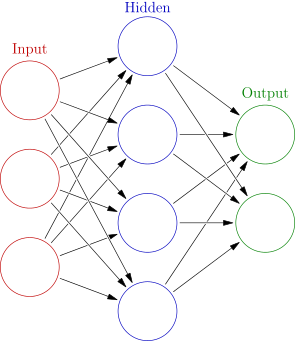
\includegraphics[scale=0.5]{simple_ann.png}
\end{figure}

\subsection{Convolutional Neural Networks}
Write about conv nets, their performance, history etc

\subsection{Training}
Write about training nets, loss functions, optimisers etc

\subsection{Prediction}
Write about generating predictions from the networks

\subsection{Performance Measures}
Write about performance measures - ROC curve, Cohen's Kappa etc
Discuss train vs valid performance, overfitting etc.

\subsection{State-of-the-Art}
What is the current image processing SOTA - e.g. ILSVRC
Anything done specifically for radiology?

\subsection{Pretrained Models}
Discuss the use of pre-trained models - can keep weights the same, replact the head.
Describe the structure of the pre-trained models we'll use for comparison:
[MAYBE PUT INTO APPENDIX?] 
\subsubsection{VGG16}
Describe VGG16 \\

% END BACKGROUND


% BEGIN DATA
\newpage
\section{Data}
Write about the MURA data, show some exmaple images (normal \& abnormal), give data breakdowns 

\subsection{MURA}
Discuss MURA - what it is, how it was produced

\subsection{Image Examples}
As can be seen in \textbf{Figure \ref{fig:xray1}} below, the x-ray is of a hand. A side-profile of the hand from the same study can be seen in \textbf{Figure \ref{fig:xray2}}. \textbf{Figure \ref{fig:xray2_copy}} is a copy of \textbf{Figure \ref{fig:xray2}}.

\begin{figure}
  \centering    
  \caption{Example X-Ray Image}
  \label{fig:xray1}
  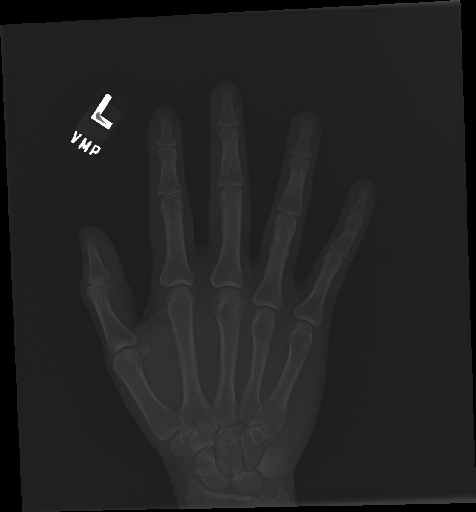
\includegraphics[scale=0.5]{image1.png}
  \caption{Another example X-Ray Image}
  \label{fig:xray2}
  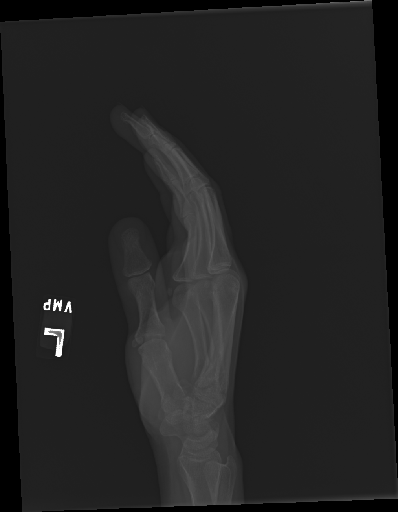
\includegraphics[scale=0.5]{image2.png}
  \caption{A copy of figure 2}
  \label{fig:xray2_copy}
  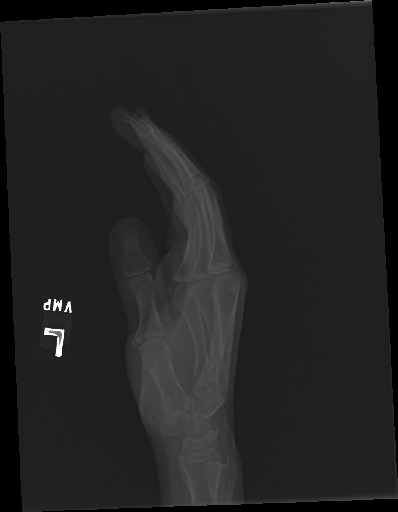
\includegraphics[scale=0.5]{image2_copy.png}
\end{figure}
\clearpage
\noindent

\subsection{Data Breakdowns}
Data breakdowns

% END DATA


% BEGIN MODEL DEVELOPMENT
\newpage
\section{Model Development}

\subsection{Working Environment}
Describe google cloud set-up, GPU, python packages used etc

\subsection{Data Preprocessing}
Describe the preprocessing work done on the data - resize images, normalise values, data augmentation etc 

\subsection{Model}
Describe the final ab-initio model I end up with - structure, loss function, training params/hyperparams etc

\subsection{Predictions}
Discuss getting predictions and aggregating down to study-level predctions

% END MODEL DEVELOPMENT


% BEGIN RESULTS
\newpage
\section{Results}

\subsection{Baseline Performance}
Give the performance of my chosen ab-initio model

\subsection{Image Size}
How do my results vary with size of image? Does increasing image size increase scope for

\subsection{Regularisation}
Perform some regularisation experiments, show results

\subsection{Pre-Trained Models}
How does my model compare vs a selection of pretrained models

% END RESULTS


% BEGIN CONCLUSIONS
\newpage
\section{Conclusions}
Include introspective chapter
Work here not comaparable to clinical setting, e.g. smaller, lower resoution images; radiologist may have a relationship with patient - know medical history, other symptoms etc
What is "abnormal"? - type \& severity of abnormality not known, MURA paper not clear.

% END CONCLUSIONS


% BEGIN ETHICAL
\newpage
\section{Professional and Ethical Issues}
Potential Impact on Radiology - Deep Learning tools used to help triage/prioritise radiologists' work, not replace them; 
Can we trust diagnosis to a computer program? Would you be happy to do so? 
Conversely - medical errors happen a lot (est. cost \$X p.a.; any specifics for radiology?) but DL tools may at least help cut that down.

% END ETHICAL


% BEGIN EXTENSIONS
\newpage
\section{Extensions}
Enquire further about what "abnormal" means
Alternative data e.g. CheXNet, others(?)
Alter NN to accept multiple images simultaneously and so predict based on several views at once (e.g. by weight-sharing, or appening all study images into a single 3D tensor)

% END EXTENSIONS



\clearpage
\bibliographystyle{plain}
\bibliography{bibliography}

\clearpage
\appendix
\section{Pretrained Model Architechtures}
Below we describe the architechtures of the various pre-trained neural network models mentioned in the text.
\subsection{VGG16}
This is the VGG16 model.


\end{document}
